\documentclass[10pt, aspectratio=169]{beamer}

\usepackage[T1]{fontenc}

\usepackage[UTF8,fontset=none]{ctex}
\setCJKmainfont[
  Path=/System/Library/AssetsV2/com_apple_MobileAsset_Font8/86ba2c91f017a3749571a82f2c6d890ac7ffb2fb.asset/AssetData/,
  FontIndex=3,
  AutoFakeBold=2
]{PingFang.ttc}
\setCJKsansfont[
  Path=/System/Library/AssetsV2/com_apple_MobileAsset_Font8/86ba2c91f017a3749571a82f2c6d890ac7ffb2fb.asset/AssetData/,
  FontIndex=3,
  AutoFakeBold=2
]{PingFang.ttc}
\setCJKmonofont[
  Path=/System/Library/AssetsV2/com_apple_MobileAsset_Font8/86ba2c91f017a3749571a82f2c6d890ac7ffb2fb.asset/AssetData/,
  FontIndex=3,
  AutoFakeBold=2
]{PingFang.ttc}
\usetheme[
  titlepage=moloch,
  sectionpage=none,
  progressbar=frametitle,
]{moloch}

\setbeamertemplate{page number in head/foot}[appendixframenumber]
\setbeamertemplate{section in toc}[sections numbered]

\usepackage{booktabs}
\usepackage[scale=2]{ccicons}

\usepackage[semibold,light]{FiraSans}
\usepackage{FiraMono}

\usepackage{xspace}

\title{近似计算在 VLA 中的应用与优化}
\subtitle{以 \texorpdfstring{$\pi_0$}{pi0} 为例}
\date{\today}
\author{傅逸凡}
\institute{电气工程学院, 西南交通大学}
\titlegraphic{\IfFileExists{assets/logo.pdf}{\hfill
\includegraphics[width=3.5cm]{assets/logo.pdf}}{}}

\begin{document}

\maketitle

\begin{frame}
  \frametitle{目录}
  \tableofcontents[hideallsubsections]
\end{frame}

\section{引言}

\begin{frame}
  \frametitle{研究切入点}
  \begin{columns}[T,onlytextwidth]
    \column{0.5 \textwidth}
    \begin{block}{$\pi_0$ 的模型特点}
      \small
      在视觉--语言模型的基础上，$\pi_0$ 进一步面向机器人控制任务，
      其核心区别在于：
      \begin{itemize}
        \item Prefix-Suffix 推理模式；
              % 图像语言 prefix 主要由 VLM backbone 处理并可缓存；状态和动作 suffix 由 action expert 在 flow matching 中反复计算，因此 FPGA 优化重点应放在 suffix/action expert 中重复出现的 Linear、Attention 和 MLP。
        \item Flow Matching 多步迭代推理；
              % π0 不是一次 forward 直接输出结果，而是通过 10 步左右的 denoising / Euler 更新生成动作。
              % 近似计算收益会被重复调用放大，flow steps 数量本身也可成为优化变量。
        \item 连续动作 token 带来的数值精度敏感性；
              % 输出是连续动作向量，不是离散文本 token，因此量化误差不能只看分类准确率或 top-k，而要看向量误差、cosine similarity、轨迹偏差等。
              % → 误差评估指标需要从 NLP 指标转向数值/控制相关指标。
      \end{itemize}
    \end{block}
    \begin{alertblock}{研究重点：从架构瓶颈到近似计算}
      \small
      本研究包含如下内容：
      \begin{itemize}
        \item \textbf{$\pi_0$建模、理论推导：} 分析部署瓶颈、给出近似计算优化方案；
        \item \textbf{$PyTorch$实验：} 通过量化和神经网络替代方法验证优化方案的有效性；
        \item \textbf{$Vitis HLS$测试：} 实现关键模块，评估资源占用、性能提升和误差影响；
      \end{itemize}
    \end{alertblock}
    \column{0.43\textwidth}
    \begin{exampleblock}{原题（概括）}
      \footnotesize
      \vspace{6pt}
      \textbf{任务一：分析 $\pi_0$ 推理架构与 FPGA 部署瓶颈。} \\
      说明推理阶段的数据流：图像经 ViT 等视觉编码器提取特征，再由投影网络映射到语言模型嵌入空间，作为视觉 token 参与后续生成。\\
      \vspace{2pt}
      结合 FPGA 的 LUT、BRAM、DSP 等资源，分析矩阵乘法与注意力计算复杂度高、模型参数和中间激活占用存储大、片外访存带宽压力大，以及定点化精度控制困难等问题。\\
      \vspace{6pt}
      \textbf{任务二：设计一种面向 $\pi_0$ 的近似计算优化方案。} \\
      量化方向：对视觉编码器、投影层和语言模型中的 Linear、Attention、FFN 等模块进行 INT8/INT4 或混合精度量化，利用 FPGA DSP 定点乘加加速；\\
      \vspace{2pt}
      神经网络替代方向：用分段线性函数、查表法或低秩近似替代复杂非线性激活、高维矩阵运算或部分注意力计算，并评估误差与硬件资源收益。
    \end{exampleblock}
  \end{columns}
\end{frame}

\begin{frame}
  \frametitle{$\pi_0$模型数据流}
  \centering
  \IfFileExists{assets/pi0_vla_flow_model.pdf}{%
    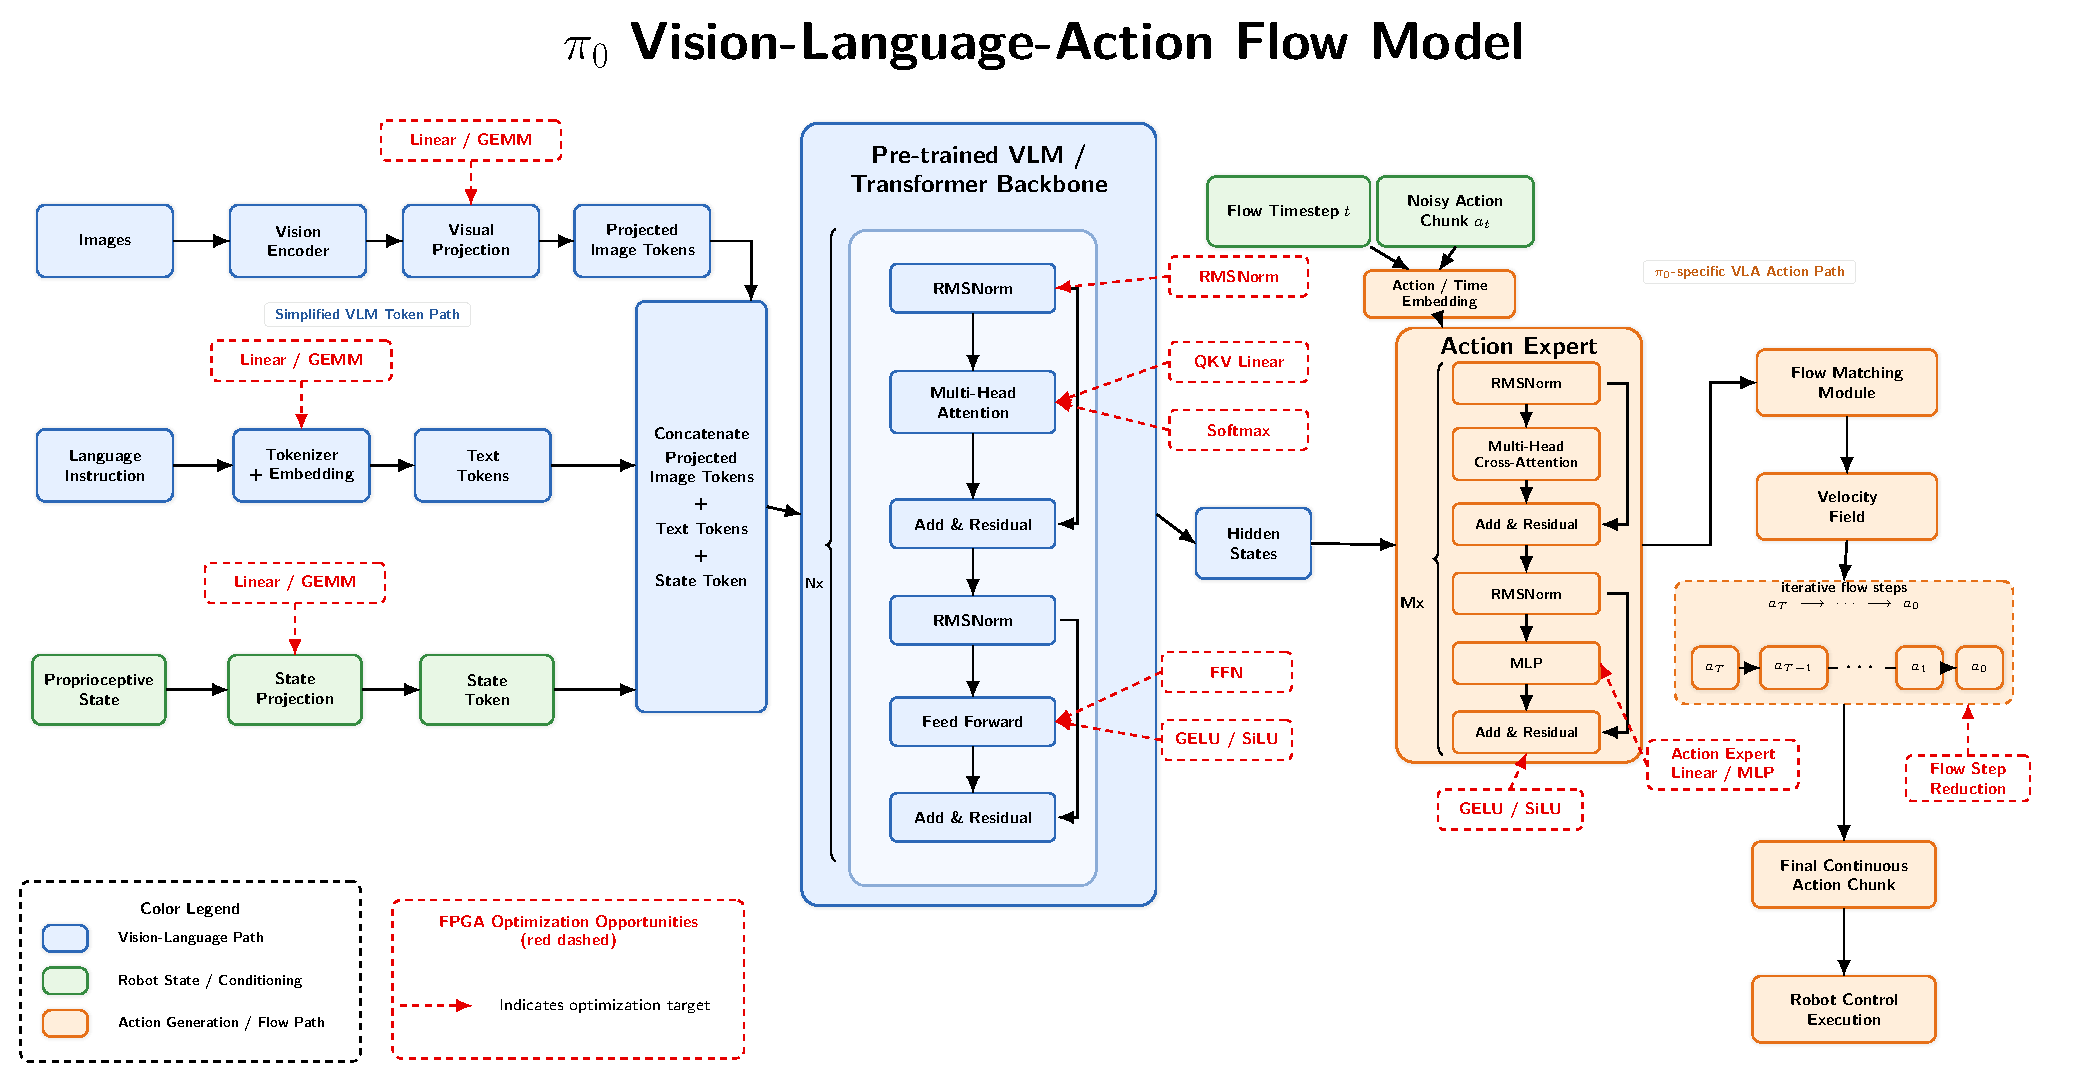
\includegraphics[width=.96\textwidth,height=.90\textheight,keepaspectratio]{assets/pi0_vla_flow_model.pdf}%
  }{%
    \IfFileExists{assets/pi0_vla_flow_model.png}{%
      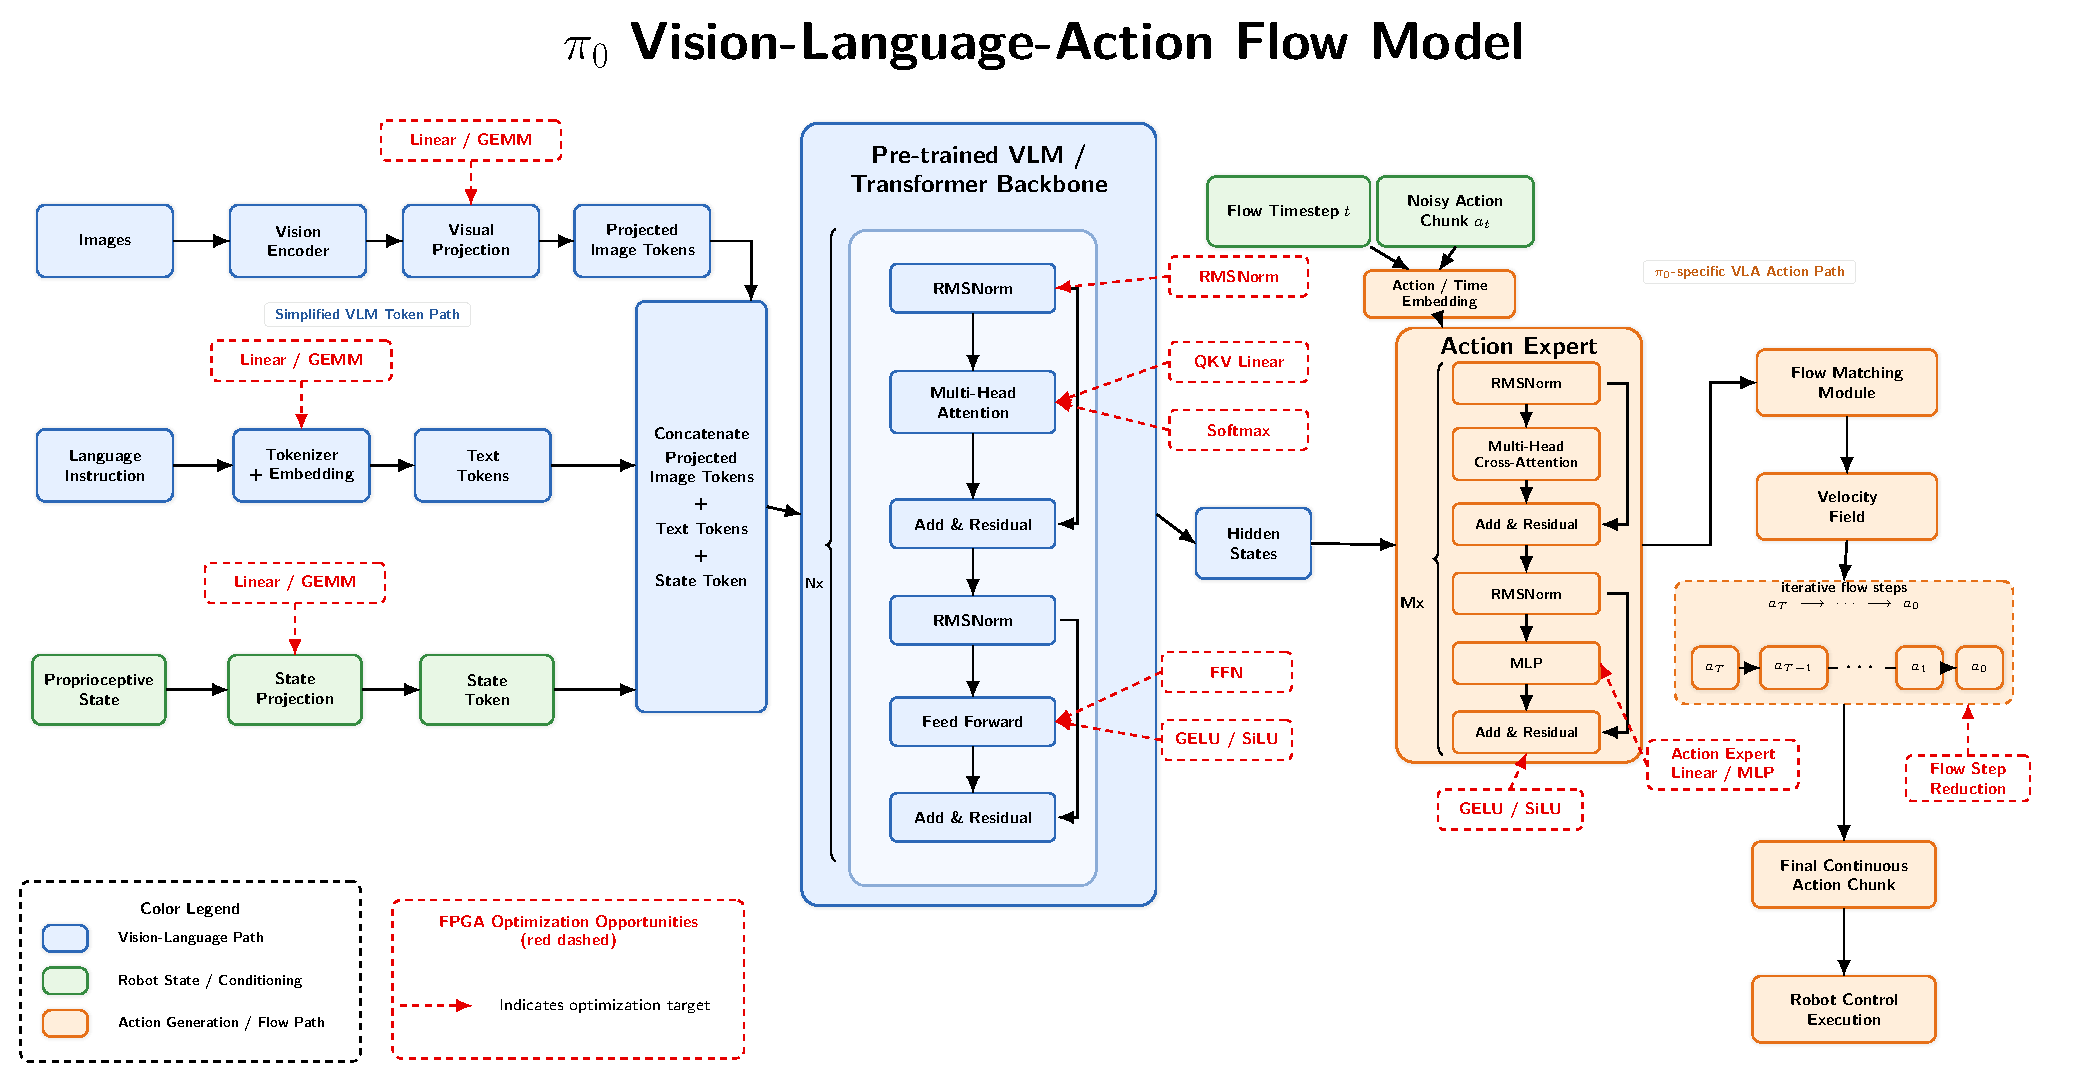
\includegraphics[width=.96\textwidth,height=.90\textheight,keepaspectratio]{assets/pi0_vla_flow_model.png}%
    }{%
      \IfFileExists{pi0_vla_flow_model.png}{%
        
\includegraphics[width=.96\textwidth,height=.90\textheight,keepaspectratio]{pi0_vla_flow_model.png}%
      }{%
        \begin{alertblock}{缺少架构图文件}
          请将 \texttt{pi0\_vla\_flow\_model.pdf} 或 \texttt{pi0\_vla\_flow\_model.png} 放入 \texttt{assets/} 目录。
        \end{alertblock}%
      }%
    }%
  }
  % 图中 Linear/GEMM 以 visual projector 为例，实际还包括 state/action projection、QKV/O projection、FFN 以及 action expert MLP 中的大量矩阵乘。
\end{frame}


\section{任务一：分析\texorpdfstring{$\pi_0$}{pi0}推理架构与FPGA部署瓶颈}

\begin{frame}
  \frametitle{任务一：FPGA 部署瓶颈总览}
  \small
  \begin{columns}[T,onlytextwidth]
    \column{0.49\textwidth}
    \begin{block}{不是单一算子问题}
      $\pi_0$ 的瓶颈来自完整推理链路叠加：
      \begin{itemize}
        \item 模型规模与片外访存；
        \item 多视角视觉 token 膨胀；
        \item Transformer GEMM / Attention；
      \end{itemize}
    \end{block}

    \column{0.47\textwidth}
    \begin{block}{VLA 额外困难}
      与普通 VLM 相比，机器人动作链路还引入：
      \begin{itemize}
        \item Softmax / GELU / SiLU / RMSNorm；
        \item flow matching 多步迭代；
        \item 连续状态和动作的定点精度敏感性。
      \end{itemize}
    \end{block}
  \end{columns}

  \vspace{4pt}
  \begin{alertblock}{核心结论}
    完整 $\pi_0$ 不适合直接部署到资源受限 FPGA；
    更合理的路线是抽取 projector、Linear/GEMM、attention softmax、
    norm/activation 和 action expert 小模块做近似计算与 HLS kernel 验证。
  \end{alertblock}
\end{frame}

\begin{frame}
  \frametitle{瓶颈一：模型规模、访存与视觉 token}
  \small
  \begin{columns}[T,onlytextwidth]
    \column{0.48\textwidth}
    \begin{block}{模型规模较大}
      $\pi_0$ 基于约 3B 级 PaliGemma VLM，
      并加入约 300M 参数的 action expert，
      即使量化到 INT4，权重规模也在 GB 级。\\
      % 总规模约 3.3B 参数。
      % openpi README 对推理显存的估计也在 8GB 以上。
      \vspace{4pt}
      \setlength{\tabcolsep}{5pt}
      \begin{tabular}{@{}lrr@{}}
        \toprule
        精度        & Bytes/param & 权重规模    \\
        \midrule
        FP32      & 4.0         & 13.2 GB \\
        FP16/BF16 & 2.0         & 6.6 GB  \\
        INT8      & 1.0         & 3.3 GB  \\
        INT4      & 0.5         & 1.65 GB \\
        \bottomrule
      \end{tabular}
    \end{block}
    \column{0.48\textwidth}
    \begin{block}{模型应用场景决定token数量大}
      PaliGemma 由 SigLIP image encoder、Gemma decoder
      和线性投影层组成。不同分辨率会产生固定 image tokens：\\
      \vspace{4pt}
      \begin{tabular}{@{}lrrr@{}}
        \toprule
        场景      & tokens & $T^2$ score & 相对 224 单图     \\
        \midrule
        224 单图  & 256    & 65K         & 1.0$\times$   \\
        224 三相机 & 768    & 589K        & 9.0$\times$   \\
        448 单图  & 1024   & 1.05M       & 16.0$\times$  \\
        448 三相机 & 3072   & 9.44M       & 144.0$\times$ \\
        896 单图  & 4096   & 16.78M      & 256.0$\times$ \\
        \bottomrule
      \end{tabular}
    \end{block}
    \vspace{6pt}
  \end{columns}
  \begin{columns}[T,onlytextwidth]
    \column{0.48\textwidth}
    \begin{alertblock}{模型规模与访存压力}
      权重难以完整放入 BRAM/URAM；
      须频繁从 DDR/HBM 搬运权重，
      导致高延迟和带宽压力。
    \end{alertblock}
    \column{0.48\textwidth}
    \begin{exampleblock}{应用场景压力}
      多相机 + 高分辨率 + ViT token 化，
      会按 $T^2$ 放大 attention score、softmax 和片上缓存压力。
    \end{exampleblock}
  \end{columns}
\end{frame}

\begin{frame}
  \frametitle{瓶颈二：算子类型与 FPGA 优势不匹配}
  \footnotesize
  \begin{table}
    \setlength{\tabcolsep}{3pt}
    \renewcommand{\arraystretch}{1.25}
    \begin{tabular}{@{}p{0.3\linewidth}p{0.32\linewidth}p{0.36\linewidth}@{}}
      \toprule
      $\pi_0$ 中的位置                  & 涉及的算子类型                        & FPGA 不擅长之处                                           \\
      \midrule
      SigLIP / PaliGemma 图像 token   & ViT attention softmax          & $QK^T$ 后有 exp、reduce-sum、division；token 增加还会放大片上缓存压力 \\
      Gemma / action expert 注意力     & masked softmax、attention map   & 动态 score 矩阵和归一化不易流式化，attention map 难完全驻留片上           \\
      Gemma MLP / action expert MLP & GELU / SiLU / gated activation & 非线性激活不是 FPGA 最擅长的规则乘加，定点误差会影响连续动作输出                  \\
      各 Transformer block           & RMSNorm / LayerNorm            & square、mean、rsqrt 或 division 形成归约和倒数平方根瓶颈            \\
      位置与时间条件注入                     & RoPE、timestep embedding        & sin/cos、逐元素旋转和广播混合，控制逻辑比单纯 GEMM 更零散                  \\
      Flow Matching 迭代采样            & 多步 denoising / Euler update    & 单步算子不复杂，但重复调用会放大上述非线性与归约算子的延迟                        \\
      \bottomrule
    \end{tabular}
  \end{table}

  \vspace{3pt}
  \begin{block}{核心矛盾}
    FPGA 的高效区间是规则、可流水、可定点化的乘加阵列；
    $\pi_0$ 的关键路径却混入 softmax、Norm、激活函数和位置/时间编码等
    非规则算子。
  \end{block}
\end{frame}

\begin{frame}
  \frametitle{瓶颈三：定点加速与连续动作误差}
  \small
  \begin{block}{核心矛盾}
    FPGA 的高吞吐来自低比特定点乘加；但 $\pi_0$ 输出的是连续 action chunk，
    量化误差会沿 flow matching 的多步更新进入机器人轨迹。
  \end{block}

  \vspace{2pt}
  \begin{columns}[T,onlytextwidth]
    \column{0.49\textwidth}
    \begin{exampleblock}{FPGA擅长量化计算}
      INT8/INT16 更适合 DSP 并行展开，
      权重、KV cache 和中间激活的片上存储压力也会下降。\\
      \vspace{3pt}
      但 $\pi_0$ 的 action expert 在一次动作生成中要被重复调用；
      论文实验使用 10 个 integration steps，
      所以单步量化收益会被多步推理放大。
    \end{exampleblock}

    \column{0.47\textwidth}
    \begin{alertblock}{为什么 $\pi_0$ 难量化}
      推理时动作由 Euler 更新得到：
      \[
        A_t^{\tau+\delta}=A_t^\tau+\delta v_\theta(A_t^\tau,o_t)
      \]
      若定点化引入 $e_q$：
      \[
        \hat A_t^{\tau+\delta}
        =\hat A_t^\tau+\delta\{v_\theta(\hat A_t^\tau,o_t)+e_q\}
      \]
    \end{alertblock}

    \vspace{2pt}
    文本 logits 只需保持排序大体正确；
    连续动作误差会直接变成轨迹偏差，
    多步迭代后可能表现为抖动、漂移或饱和。
  \end{columns}
\end{frame}

\section{任务二：近似计算方案与实验设计}

\begin{frame}
  \frametitle{改进策略：哪些模块最值得近似计算}
  \footnotesize
  \begin{table}
    \renewcommand{\arraystretch}{1.25}
    \setlength{\tabcolsep}{3pt}
    \begin{tabular}{@{}p{0.24\linewidth}p{0.42\linewidth}p{0.3\linewidth}@{}}
      \toprule
      模块                     & FPGA 部署瓶颈                 & 近似优化切入点                        \\
      \midrule
      Q/K/V/O Linear         & 大量矩阵乘，DSP 与权重带宽占用高        & INT8 / W4A8 tiled GEMM         \\
      Attention Score $QK^T$ & 序列长度增加后呈二次复杂度             & 分块、低比特 score                   \\
      Softmax                & exp、sum、division 对硬件不友好   & LUT、PWL、Taylor、base-2          \\
      FFN / MLP              & Transformer 中最大 GEMM 来源之一 & INT8 GEMM、低秩/剪枝                \\
      GELU / SiLU            & tanh / sigmoid 等非线性成本高    & LUT / PWL / hard approximation \\
      RMSNorm                & 涉及平方、均值、倒数平方根             & fixed-point + rsqrt            \\
      Flow Matching          & action expert 多步重复调用      & 减少 Euler steps                 \\
      \bottomrule
    \end{tabular}
  \end{table}

  \vspace{3pt}
  \begin{alertblock}{本项目策略}
    先用 PyTorch 判断误差风险，再把有价值的算子落到 Vitis HLS，得到 latency、II、LUT、FF、BRAM、DSP 等硬件指标。
  \end{alertblock}
\end{frame}

\begin{frame}
  \frametitle{任务二：面向 $\pi_0$ 的模块级近似计算方案}
  \small
  \begin{table}
    \begin{tabular}{@{}p{0.25\linewidth}p{0.37\linewidth}p{0.28\linewidth}@{}}
      \toprule
      优化对象               & 近似/定点化方法                                             & 预期收益                  \\
      \midrule
      Linear / QKV / FFN & INT8、INT4、W4A8 fake quant；INT32/INT24 累加后 requantize & 降低 GEMM 计算和权重存储       \\
      Softmax            & LUT、PWL、Taylor、base-2 softmax                        & 避免高成本 exp/div         \\
      GELU / SiLU        & PWL、hard approximation、clipped linear                & 降低复杂激活函数开销            \\
      RMSNorm            & fixed-point + reciprocal sqrt 近似                     & 降低 sqrt/div 成本        \\
      Flow steps         & 10 steps $\rightarrow$ 8/6/4/2 steps                 & 减少 action expert 调用次数 \\
      \bottomrule
    \end{tabular}
  \end{table}

  \vspace{4pt}
  \begin{exampleblock}{FPGA 适配}
    Vitis HLS 的 arbitrary precision 与 fixed-point 类型可以直接指定位宽。
    因此 INT8、INT16 和定点 rsqrt/LUT 都能对应到更小的乘加单元、片上缓存和查表逻辑。
  \end{exampleblock}
\end{frame}


\begin{frame}
  \frametitle{实验工作量总览：从算法误差到 HLS 可综合验证}
  \small
  \begin{columns}[T,onlytextwidth]
    \column{0.52\textwidth}
    \begin{block}{PyTorch 侧：模块误差与趋势评估}
      \scriptsize
      基础算子：Linear / projector / softmax / GELU / RMSNorm。\\
      \vspace{2pt}
      模型对齐：scale sweep、$\pi_0$-aligned random proxy、
      real-weight + random input。\\
      \vspace{2pt}
      算法旋钮：$\pi_0$-shape toy flow step reduction。
    \end{block}

    \column{0.44\textwidth}
    \begin{alertblock}{Vitis HLS 侧：硬件可实现性验证}
      \scriptsize
      近似 kernel：INT8 GEMM、LUT softmax、PWL GELU、
      RMSNorm rsqrt、fixed-point projector tile。\\
      \vspace{2pt}
      对比基线：exact softmax / GELU / RMSNorm。\\
      \vspace{2pt}
      输出指标：latency、II、clock、LUT、FF、BRAM、DSP。
    \end{alertblock}
  \end{columns}

  \vspace{3pt}
  \begin{exampleblock}{主要输出}
    CSV / figures / HLS report / kernel summary / before-after comparison，
    形成“误差趋势 $\rightarrow$ 可综合验证”的闭环。
  \end{exampleblock}
\end{frame}

\section{PyTorch 实验结果}

\begin{frame}
  \frametitle{PyTorch 实验设计：从随机张量到真实权重}
  \small
  \begin{columns}[T,onlytextwidth]
    \column{0.61\textwidth}
    \begin{block}{实验分层}
      \scriptsize
      \setlength{\tabcolsep}{2pt}
      \begin{tabular}{@{}p{0.28\linewidth}p{0.18\linewidth}p{0.22\linewidth}p{0.20\linewidth}@{}}
        \toprule
        层级           & 输入            & 权重         & 目的        \\
        \midrule
        Random shape & random tensor & random     & 看趋势       \\
        Real weight  & random tensor & checkpoint & 看误差       \\
        Toy flow     & 合成 action     & 小模型        & 看 step 权衡 \\
        \bottomrule
      \end{tabular}
    \end{block}

    \begin{exampleblock}{评价指标}
      MSE、MAE、max error、cosine similarity、relative L2、KL divergence、latency、weight size、compression ratio。
    \end{exampleblock}

    \column{0.35\textwidth}
    \begin{alertblock}{限制}
      这些实验是模块级验证，用来判断近似方向是否值得继续做 HLS kernel；
      它不等于端到端机器人控制评估。
    \end{alertblock}
  \end{columns}
\end{frame}


\begin{frame}
  \frametitle{实验结果一：GEMM 类模块适合优先 INT8 定点化}
  \small
  \begin{columns}[T,onlytextwidth]
    \column{0.58\textwidth}
    \begin{table}
      \scriptsize
      \setlength{\tabcolsep}{2pt}
      \begin{tabular}{@{}p{0.37\linewidth}cc@{}}
        \toprule
        实验设置                   & INT8 最低 cosine & INT4 最低 cosine \\
        \midrule
        $\pi_0$-aligned random & 0.998402       & 0.963150       \\
        real $\pi_0$ weight    & 0.994843       & 0.921080       \\
        \bottomrule
      \end{tabular}
    \end{table}

    \begin{exampleblock}{观察}
      INT8 在随机结构和真实权重实验中都比较稳。
      INT4 / W4A8 压缩更强，但误差上升更明显。
    \end{exampleblock}

    \column{0.38\textwidth}
    \begin{alertblock}{FPGA 侧优先级}
      \footnotesize
      优先对象：projector、QKV、FFN、动作投影、action expert。\\
      实现方向：INT8 tiled GEMM。INT4 更适合作为激进压缩选项。
    \end{alertblock}
  \end{columns}
\end{frame}

\begin{frame}
  \frametitle{实验结果二：Softmax / RMSNorm 可近似，激活替换需谨慎}
  \small
  \begin{columns}[T,onlytextwidth]
    \column{0.32\textwidth}
    \begin{block}{Softmax}
      LUT softmax 在真实 Q/K score 上 relative L2 约为 $4.3\times10^{-5}$，
      已迁移到 HLS LUT kernel 验证。
    \end{block}

    \column{0.32\textwidth}
    \begin{block}{RMSNorm}
      真实权重实验中 RMSNorm 近似最大 relative L2 约为 0.0117，
      可继续做 fixed-point + rsqrt。
    \end{block}

    \column{0.32\textwidth}
    \begin{alertblock}{GELU / SiLU}
      identity 或过激 clipped-linear 替换可能让 relative L2 接近 1。
      激活函数不能粗暴替换。
    \end{alertblock}
  \end{columns}

  \vspace{4pt}
  \begin{exampleblock}{结论}
    Softmax 与 RMSNorm 的近似比较可控；GELU/SiLU 要放回完整 FFN 里评价，优先采用保守 PWL/LUT。
  \end{exampleblock}
\end{frame}

\begin{frame}
  \frametitle{实验结果三：Flow Step Reduction 算法级加速}
  \small
  \begin{columns}[T,onlytextwidth]
    \column{0.50\textwidth}
    \begin{block}{实验设置}
      \begin{itemize}
        \item $\pi_0$ 链路：noisy action $\rightarrow$ multi-step flow integration $\rightarrow$ clean action chunk；
        \item toy flow matching：$H=50$, action dim $=32$；
        \item 对比 10 / 8 / 6 / 4 / 2 step Euler integration。
      \end{itemize}
    \end{block}

    \column{0.46\textwidth}
    \begin{exampleblock}{观察}
      2-step 相比 10-step 约 $4.46\times$ 加速，MSE 约 $4.32\times10^{-3}$，cosine 约 0.9975。
    \end{exampleblock}

    \begin{alertblock}{限制}
      这部分说明减少 flow step 有潜在加速收益。
      真实动作质量仍需要 observation / action trajectory 和任务成功率验证。
    \end{alertblock}
  \end{columns}
\end{frame}

\section{Vitis HLS 实验结果}

\begin{frame}
  \frametitle{Vitis HLS 实验：关键模块可综合验证}
  \small
  \begin{table}
    \scriptsize
    \setlength{\tabcolsep}{2pt}
    \begin{tabular}{@{}p{0.22\linewidth}p{0.30\linewidth}p{0.38\linewidth}@{}}
      \toprule
      HLS kernel & 对应 $\pi_0$ 模块 & 验证内容 \\
      \midrule
      INT8 GEMM & projector / QKV / FFN / action projection & INT8 乘加、INT32 累加、INT16 requantize \\
      LUT softmax & attention score normalization & max-subtraction、clamp、LUT exp、归一化 \\
      PWL GELU & FFN / action expert activation & 16 段 PWL 近似，替代 tanh GELU \\
      RMSNorm rsqrt & Transformer / action expert norm & fixed-point + LUT 初始化 + Newton-Raphson \\
      fixed projector tile & visual projector tile & $[64,1152]\rightarrow[64,256]$ 定点 projector \\
      exact baselines & softmax / GELU / RMSNorm & 用于 before/after 对比 \\
      \bottomrule
    \end{tabular}
  \end{table}

  \begin{exampleblock}{验证指标}
    C-sim 数值误差 + C-synthesis 报告：latency、II、estimated clock、LUT、FF、BRAM、DSP。
  \end{exampleblock}
\end{frame}

\begin{frame}
  \frametitle{HLS 结果一：延迟、资源与数值误差}
  \scriptsize
  \begin{table}
    \setlength{\tabcolsep}{2pt}
    \begin{tabular}{@{}p{0.16\linewidth}p{0.20\linewidth}rrrrrp{0.20\linewidth}@{}}
      \toprule
      Kernel & Shape & Latency & LUT & FF & BRAM & DSP & 误差指标 \\
      \midrule
      INT8 GEMM & $50\times32\times1024$ & 1,742,214 & 6,953 & 4,024 & 19 & 5 & MSE=0, cosine=1.0 \\
      LUT Softmax & rows4 len128 & 1,867 & 3,692 & 2,727 & 9 & 2 & KL=1.75e-3, cos=0.9993 \\
      PWL GELU & len4096 & 4,114 & 2,301 & 1,806 & 1 & 2 & rel-L2=3.07e-3 \\
      RMSNorm rsqrt & hidden1024 & 2,080 & 5,649 & 3,857 & 2 & 64 & cos $>0.9999998$ \\
      \bottomrule
    \end{tabular}
  \end{table}

  \vspace{3pt}
  \begin{alertblock}{结论}
    HLS 结果证明：选定近似对象不是停留在 PyTorch 仿真层面，
    而是可以形成可综合 kernel，并能输出 FPGA 资源与延迟报告。
  \end{alertblock}
\end{frame}

\begin{frame}
  \frametitle{HLS 结果二：exact baseline vs approximate kernel}
  \scriptsize
  \begin{table}
    \setlength{\tabcolsep}{2pt}
    \begin{tabular}{@{}p{0.16\linewidth}p{0.22\linewidth}p{0.20\linewidth}p{0.15\linewidth}p{0.19\linewidth}@{}}
      \toprule
      对比对象 & baseline & approximate & 时间收益 & 资源变化 \\
      \midrule
      Softmax & float exp softmax & LUT softmax & $1.92\times$ & DSP $-85.7$，LUT $-10.7$ \\
      GELU & float tanh GELU & 16-seg PWL GELU & $1.01\times$ & LUT $-70.7$，DSP $-96.7$ \\
      RMSNorm & float sqrt RMSNorm & rsqrt + NR & $2.09\times$ & LUT $+54.5$，DSP $+540$ \\
      \bottomrule
    \end{tabular}
  \end{table}

  \begin{exampleblock}{分析}
    Softmax 和 GELU 的近似替换资源收益明显；
    当前 RMSNorm rsqrt 主要改善 estimated clock/time，
    但 DSP 代价偏高，后续应优化 LUT/NR 数据通路或降低并行度。
  \end{exampleblock}
\end{frame}

\begin{frame}
  \frametitle{实验闭环：PyTorch 负责选方向，HLS 负责证实可实现}
  \small
  \begin{columns}[T,onlytextwidth]
    \column{0.47\textwidth}
    \begin{block}{PyTorch 侧回答}
      \footnotesize
      INT8 在 random、$\pi_0$-aligned 和 real-weight 下均较稳；
      INT4/W4A8 压缩强但真实权重误差偏高。\\
      \vspace{2pt}
      LUT softmax、RMSNorm rsqrt 误差可控；
      激进 activation replacement 风险高；
      flow step reduction 有潜在加速收益。
    \end{block}

    \column{0.49\textwidth}
    \begin{alertblock}{HLS 侧回答}
      \footnotesize
      INT8 GEMM 可综合，面向 projector / QKV / FFN / action projection。\\
      \vspace{2pt}
      LUT softmax 明显减少 DSP；
      PWL GELU 明显减少 LUT/DSP。\\
      \vspace{2pt}
      RMSNorm rsqrt 误差很小，但当前实现资源仍需优化。
    \end{alertblock}
  \end{columns}

  \vspace{3pt}
  \begin{exampleblock}{闭环结论}
    推荐主线：INT8 GEMM + LUT softmax + 保守 PWL GELU + fixed-point RMSNorm；
    flow step reduction 作为算法级优化旋钮单独讨论。
  \end{exampleblock}
\end{frame}

\section{总结}

\begin{frame}
  \frametitle{总结与边界}
  \small
  \begin{enumerate}
    \item \textbf{架构层面：} $\pi_0$ 是 VLM backbone + action expert + flow matching，完整上板不现实，应拆成可优化模块。
    \item \textbf{PyTorch 层面：} 已完成 random shape、real-weight proxy 和 toy flow step reduction；INT8 是当前最稳的 GEMM 类量化方案。
    \item \textbf{HLS 层面：} 已实现并综合 INT8 GEMM、LUT softmax、PWL GELU、RMSNorm rsqrt 和 fixed projector tile，获得 latency、II、LUT、FF、BRAM、DSP 数据。
    \item \textbf{方案判断：} Softmax/GELU 近似在 HLS 中资源收益明显；RMSNorm 误差较小但当前 DSP 代价偏高；INT4/W4A8 和激进 activation replacement 需谨慎。
  \end{enumerate}

  \begin{block}{总结}
    本次工作不是复现完整 $\pi_0$，而是把 VLA 推理链路拆成可在 FPGA 上验证的关键模块，并完成从 PyTorch 误差评估到 Vitis HLS 可综合报告的闭环验证。
  \end{block}

  \vspace{10pt}

  \centering
  \small 谢谢老师，请批评指正。
\end{frame}

\appendix

\section{Appendix}

\begin{frame}
  \frametitle{Appendix：$\pi_0$ 关键模块 Shape}
  \scriptsize
  \begin{table}
    \begin{tabular}{@{}p{0.24\linewidth}p{0.38\linewidth}p{0.30\linewidth}@{}}
      \toprule
      模块                      & 实验 shape / 结构                                                              & 对应优化点               \\
      \midrule
      Visual projector        & $[1,768,1152] \rightarrow [1,768,2048]$                                    & Linear / GEMM       \\
      VLM attention           & $q:2048\rightarrow2048$, $k/v:2048\rightarrow256$, $o:2048\rightarrow2048$ & QKV Linear, Softmax \\
      VLM FFN                 & $2048 \rightarrow 16384 \rightarrow 2048$，gated FFN                        & FFN, GELU/SiLU      \\
      Action expert FFN       & $1024 \rightarrow 4096 \rightarrow 1024$                                   & Action Expert MLP   \\
      State/action projection & $32\rightarrow1024$, $1024\rightarrow32$                                   & Linear / GEMM       \\
      RMSNorm                 & $[1,768,2048]$, $[1,50,1024]$                                              & fixed-point + rsqrt \\
      Flow matching toy       & $H=50$, action dim $=32$, steps $=10/8/6/4/2$                              & Flow Step Reduction \\
      \bottomrule
    \end{tabular}
  \end{table}
\end{frame}

\begin{frame}
  \frametitle{Appendix：真实权重 Proxy 的作用与限制}
  \small
  \begin{columns}[T,onlytextwidth]
    \column{0.48\textwidth}
    \begin{block}{作用}
      \begin{itemize}
        \item 使用 $\pi_0$ checkpoint 中真实模块权重；
        \item 反映真实参数分布下的量化误差；
        \item 比纯随机权重更接近实际模型。
      \end{itemize}
    \end{block}

    \column{0.48\textwidth}
    \begin{alertblock}{限制}
      \begin{itemize}
        \item 输入仍是 random tensor；
        \item 没有真实 activation calibration；
        \item 没有 action trajectory / success rate；
        \item 因此不等于端到端 $\pi_0$ 量化评估。
      \end{itemize}
    \end{alertblock}
  \end{columns}
\end{frame}

\end{document}
